\documentclass[aspectratio=43]{beamer}

\usepackage{mathpazo}
\usepackage{fontspec}
\usepackage{graphicx}
\usepackage{amsmath}
\usepackage{amssymb}
\usepackage{amsthm}
\usepackage{bm}
\usepackage{multirow}
\usepackage{hyperref}
\usepackage{braket}
\usepackage{bm}
\usepackage{mathrsfs}
\usepackage{slashed}
\usepackage{subfig}
\usepackage{tikz}
\usepackage{siunitx}
\usepackage[absolute,overlay]{textpos}
\usepackage[export]{adjustbox}
\usepackage{nccmath}
\usepackage{media9}

\DeclareMathOperator{\Tr}{Tr}

\definecolor{darkgreen}{rgb}{0,0.8,0}
\definecolor{darkblue}{rgb}{0,0,0.8}
\definecolor{graydarkred}{HTML}{E0ADAD}
\definecolor{graylightred}{HTML}{EFD6D6}

\usecolortheme{beaver}
\setbeamercolor*{itemize item}{fg=darkred}
\setbeamercolor*{itemize subitem}{fg=darkred}
\setbeamercolor*{enumerate item}{fg=darkred}
\setbeamercolor*{enumerate subitem}{fg=darkred}
\setbeamercolor{bibliography item}{fg=darkred}
\setbeamercolor{bibliography entry author}{fg=darkred}
\setbeamercolor{bibliography entry title}{fg=darkred}
\setbeamercolor{bibliography entry location}{fg=darkred}
\setbeamercolor{bibliography entry note}{fg=darkred}
\setbeamercolor{caption name}{fg=darkred}
\setbeamercolor{navigation symbols}{fg=graydarkred}
\setbeamercolor{navigation symbols dimmed}{fg=graylightred}
\setbeamercolor{section number projected}{bg=darkred}
\setbeamertemplate{section in toc}[square]
\defbeamertemplate*{headline}{infolines theme}
{%
  \leavevmode%
  \hbox{%
  \begin{beamercolorbox}[wd=.5\paperwidth,ht=2.65ex,dp=1.5ex,right]{section in head/foot}%
    \usebeamerfont{section in head/foot}\insertsectionhead\hspace*{2ex}
  \end{beamercolorbox}%
  \begin{beamercolorbox}[wd=.5\paperwidth,ht=2.65ex,dp=1.5ex,left]{subsection in head/foot}%
    \usebeamerfont{subsection in head/foot}\hspace*{2ex}\insertsubsectionhead{}
  \end{beamercolorbox}}%
}
\addtobeamertemplate{navigation symbols}{}{%
    \usebeamerfont{footline}%
    \usebeamercolor[fg]{footline}%
    \hspace{1em}%
    \raisebox{1.4pt}[0pt][0pt]{\insertframenumber/\inserttotalframenumber}
}

\usefonttheme{professionalfonts}
\usefonttheme{serif}
\setmainfont{EB Garamond}
\setlength{\parskip}{1em}

\usepackage{import}
\usepackage{pdfpages}
\usepackage{xcolor}
\newcommand{\incfig}[2][]{%
  \def\svgwidth{{#1}\columnwidth}
    \import{./figures/}{#2.pdf_tex}
}

\captionsetup[figure]{labelformat=empty}

\title{The Quantum Monte Carlo Simulation of Transverse Field Ising Model}
\author{Yuanxing Duan, Shixin Hu and Fangyu Xiong}
\institute{School of Physics, Peking University}
\date{January 5, 2021}

\AtBeginSection[]{
  \begin{frame}
    \frametitle{Outline}
    \tableofcontents[currentsection]
  \end{frame}
}

\begin{document}
\maketitle

\section{Introduction to Transverse Field Ising}
\begin{frame}{Classical Ising Model}
Hamiltonian:

\[
\mathcal{H}=-t\sum_{\braket{ij}}\sigma_i^z\sigma_j^z-h_z\sum_{i}\sigma_i^z
\]

Thermal Fluctuation $\Longrightarrow$ Thermal(Classical) Phase Transition
\[
\]
Low T: Ordered state

High T: Paramagnetic state
\end{frame}

\begin{frame}
\begin{figure}[htpb]
	\centering
	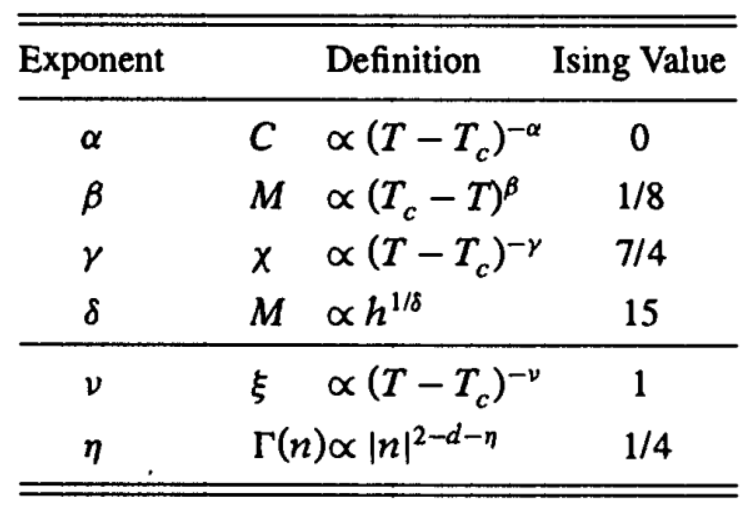
\includegraphics[width=0.6\textwidth]{figs/Critical_Exponents.png}
	\caption{Critical exponents of Classical Ising Model}
	\label{fig:Critical Exponents}
\end{figure}
\end{frame}

\begin{frame}{Quantum Ising Model}
Hamiltonian of Transverse Field Ising model (TFI):
\[
\mathcal{H}=-t\sum_{\braket{ij}}\sigma_i^z\sigma_j^z-h\sum_{i}\sigma_i^x
\]
$[\sigma_i^z,\sigma_i^x]\ne0$ $\Longrightarrow$ Quantum Fluctuation!

\[
\]

Quantum Phase Transition:

$h\ll t$: Spins aligned in z-direction.

$h\gg t$: Spins aligned in x-direction.
\end{frame}

\begin{frame}{Theoretical Calculation}

Jordan-Wigner tranformation:
\[
\sigma_i^x =1-2c^{\dagger}_ic_i
\]
\[
\sigma_i^z =-\prod_{j<i}(1-2c^{\dagger}_jc_j)(c_i+c_i^{\dagger})
\]

$c_i$s are fermion operators.
\[
\]
Hamiltonian becomes:
\[
\mathcal{H}=-t\sum_{i}(c^{\dagger}_ic_{i+1}+c^{\dagger}_{i+1}c_i+c^{\dagger}_ic^{\dagger}_{i+1}+c_{i+1}c_i-2gc^{\dagger}_ic_i+g)
\]
with $g=h/t$
\end{frame}

\begin{frame}{Theoretical Calculation}
Solve it by Bogoliubov transformation:
\[
\gamma_k=u_kc_k-v_kc_{-k}^{\dagger}
\]
\[
\gamma_k^{\dagger}=u_kc_k^{\dagger}-v_kc_{-k}
\]
with $c_k$ Fourier transformation of $c_i$. And
\[
u_k=\mathrm{cos}\left( \frac{\theta_k}{2}\right), v_k=\mathrm{sin}\left( \frac{\theta_k}{2}\right) 
\]
\[
\mathrm{tan}\left(\theta_k\right)=\frac{\mathrm{sin}(ka)}{g-\mathrm{cos}(ka)}
\]
\end{frame}

\begin{frame}{Theoretical Calculation}
Switch to Majorana representation (continuous limit):
\[
\psi(x_i)=-i(c_i-c_i^{\dagger})=\frac{1}{2N}\sum_k(u_1(k)\gamma_k^{\dagger}e^{ikx_i}+h.c.)
\]
\[
\bar{\psi}(x_i)=c_i+c_i^{\dagger}=\frac{1}{2N}\sum_k(u_2(k)\gamma_k^{\dagger}e^{ikx_i}+h.c.)
\]
\[
\psi(x_i,t)=e^{i\mathcal{H}t}\psi(x_i)e^{-i\mathcal{H}t}, \bar{\psi}(x_i,t)=e^{i\mathcal{H}t}\bar{\psi}(x_i)e^{-i\mathcal{H}t}
\]
$\Longrightarrow$ Solution of 1+1D Dirac equation
\end{frame}

\begin{frame}{Theoretical Calculation}
The action:
\[
S=\frac{i}{2}\int\psi(\partial_0-\partial_1)\psi+\bar{\psi}(\partial_0+\partial_1)\bar{\psi}+(1-g)\psi\bar{\psi}
\]
$g=1$ $\Longrightarrow$ masless, scale invariance , i.e.
\[
S^{\prime}=S \; \mathrm{when} \; x\rightarrow \lambda x
\]
$\Longrightarrow$ Critical Point at $h=t$!!
\end{frame}

\begin{frame}
The two point correlation functions at criticality:
\[
\braket{\sigma_i^z\sigma_{i+n}^z}\propto\frac{1}{|n|^{1/4}}
\]
\[
\braket{\sigma_i^x\sigma_{i+n}^x}\propto\frac{1}{|n|^2}
\]
\end{frame}

\section{Worm Algorithm}
\begin{frame}{Holstein-Primakoff Transformation}
  TFI:
  \[
    \mathcal{H} = -t\sum_{\braket{ij}}\sigma_i^x\sigma_j^x - h\sum_{i}\sigma_i^z = K+U
  \]
  Hopping and pairing terms:
  \[
    K = K_1+K_2 = -t\sum_{\braket{ij}}(\sigma_i^+\sigma_j^-+\text{h.c.})-t\sum_{\braket{ij}}(\sigma_i^+\sigma_j^++\text{h.c.})
  \]
  HP transformation: $b_i(b_i^\dag) = \sigma_i^+(\sigma_i^-)$, $n_i = b_i^\dag b_i = (\sigma_i^z+1)/2$
  \[
    \Rightarrow \mathcal{H} = -t\sum_{\braket{ij}}(b_i^\dag b_j+\text{h.c.})-t\sum_{\braket{ij}}(b_i^\dag b_j^\dag+\text{h.c.})-\mu\sum_{i}n_i
  \]
  where $\mu = 2h$.
\end{frame}

\begin{frame}{$\mathcal{Z}$ Configurations}
  \begin{align*}
    \mathcal{Z} &= \Tr \left(\mathrm{e}^{-\beta \mathcal{H}}\right) = \sum_{a_0}\bra{\alpha_0}\mathrm{e}^{-\beta \mathcal{H}}\ket{\alpha_0}\\
                &= \lim_{\mathrm{d}\tau = \frac{\beta}{n}, n \to \infty} \sum_{\{\alpha_i\}}\bra{\alpha_0}\mathrm{e}^{-\mathcal{H}\mathrm{d}\tau}\ket{\alpha_{n-1}}\cdots \bra{\alpha_i}\mathrm{e}^{-\mathcal{H}\mathrm{d}\tau}\ket{\alpha_0}\\
                &= \sum_{\alpha_0}\sum_{\mathcal{N}}^{\infty}\int_{0}^{\beta}\int_{\tau_1}^{\beta}\cdots \int_{\tau_{\mathcal{N}-1}}^{\beta} \prod_{k=1}^{\mathcal{N}}\mathrm{d}\tau_k\,F(t, h)
  \end{align*}
  \[
    F(t, h) = t^{\mathcal{N}_h+\mathcal{N}_p}\mathrm{e}^{-\int_{0}^{\beta}U(\tau)\,\mathrm{d}\tau}
  \]
  $\mathcal{N}_h$ and $\mathcal{N}_p$: number of hopping and pairing kinks. $\mathcal{N}_h + \mathcal{N}_p = \mathcal{N}$.

  $\mathcal{Z}$ configuration: several loops of spin-up (and kinks) in the $(d+1)$D space-time.\\
  Statistical weight of a $\mathcal{Z}$ configuration:
  \[
    W_{\mathcal{Z}}(t, h) = \prod_{k=1}^{\mathcal{N}}\mathrm{d}\tau\,F(t, h)
  \]
\end{frame}

\begin{frame}{$\mathcal{G}$ Configurations}
  \[
    \mathcal{G}(\bm{x}_I, \tau_I; \bm{x}_M, \tau_M) = \Tr\left[ T_\tau\left( \sigma_I^x(\tau_I)\sigma_M^x(\tau_M)\mathrm{e}^{-\beta\mathcal{H}} \right) \right]
  \]
  $\mathcal{G}$ configuration: $\mathcal{Z}$ configuration + an open path of spin-up with two ending points ``Ira'' ($I$) and ``Masha'' ($M$).

  Statistical weight of a $\mathcal{G}$ configuration:
  \[
    W_\mathcal{G} = \frac{\mathrm{d}\tau_I\mathrm{d}\tau_M}{\omega_G} \prod_{k=1}^{\mathcal{N}}\mathrm{d}\tau_k\,F(t, h)
  \]
  \begin{itemize}
    \item Key idea: move the defect $M$ of the open path to produce different $\mathcal{G}$ and $\mathcal{Z}$ configurations for sampling. (Like a worm wriggling!)
  \end{itemize}
\end{frame}

\begin{frame}{Updates}
  \vspace{-3mm}
  \begin{figure}[htpb]
    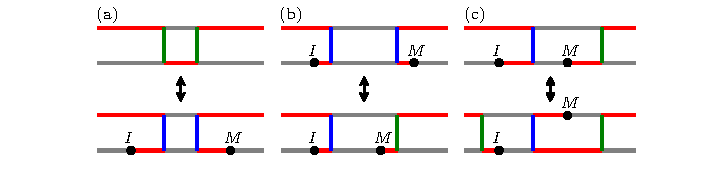
\includegraphics[width=1.2\textwidth,center]{figs/updates.pdf}
  \end{figure}
  \vspace{-9mm}
  \footnotesize
  \begin{enumerate}[(a)]
    \item Create/annihilate defects $I$ and $M$.
      {\scriptsize\useshortskip\[
        \frac{\mathrm{d}\tau_I}{\beta N}\frac{\mathrm{d}\tau_M}{\tau_a}\cdot W_\mathcal{Z}\cdot\mathcal{P}_\text{crea} = \mathcal{A}_a\cdot W_\mathcal{G}\cdot\mathcal{P}_\text{anni}
        \Rightarrow
        \begin{cases}
          P_\text{crea} = \min \left[ 1, \mathcal{A}_a \tau_a \frac{\beta N}{\omega_G}\frac{F_\text{new}}{F_\text{old}} \right]\\
          P_\text{anni} = \min\left[ 1, \frac{1}{\mathcal{A}_a \tau_a}\frac{\omega_G}{\beta N}\frac{F_\text{new}}{F_\text{old}} \right]
        \end{cases}
      \]}
    \item Move imaginary time of defect $M$.
      {\scriptsize\useshortskip\[
        P_\text{move} = \min\left\{1, \frac{F_\text{new}}{F_\text{old}}\right\}
      \]}
    \item Insert/delete a kink.
      {\scriptsize\useshortskip\[
        \mathcal{A}_c\cdot\frac{1}{z_d}\cdot\frac{\mathrm{d}\tau}{\tau_c}\cdot W\cdot \mathcal{P}_\text{inse} = \mathcal{A}_c\cdot\frac{1}{z_d}\cdot\frac{1}{n_k}\cdot W_+\cdot \mathcal{P}_\text{dele}
        \Rightarrow
        \begin{cases}
          P_\text{inse} = \min\left[1, \frac{\tau_c}{n_k+1}\frac{F_\text{new}}{F_\text{old}}\right]\\
          P_\text{dele} = \min\left[1, \frac{n_k}{\tau_c}\frac{F_\text{new}}{F_\text{old}}\right]
        \end{cases}
      \]}
  \end{enumerate}
  \vspace{-3mm}
  $\tau_a$, $\tau_b$, $\tau_c$: ranges for choosing random time displacement.\\
  \textit{A priori} probabilities: $\mathcal{A}_a+\mathcal{A}_b+2\mathcal{A}_c = 1$.
\end{frame}

\section{C++ Implement}
\begin{frame}{The Grid}
  \begin{itemize}
    \item Use one bit to represent one spin
    \item Use one bit to represent one kink between two world lines
    \item Use bitwise $\bf{XOR}$ with mask to flip spins and calculate the correlation
    \item Use $\bf{OR}$ to get the state of one spin
    \item Use bitwise $\bf{OR}$ to get the positions without kinks
    \item Use $\bf{\_\_popcnt}$ to count spin-up number
    \item Use $\bf{\_tzcnt\_u32}$ to find the first set bit to find the starting point of one loop in the grid
  \end{itemize}
\end{frame}

\begin{frame}{Warpping Number of Loops}
  \begin{itemize}
    \item Depth first search
    \item Must traverse the whole grid to find all loops and calculate the warpping number of each loop
    \item This doesn't affect the performance since its time consumption is about 1\% of creating and annihilating once
    \item Use a direction to make sure that the current point donsn't goes it way back
    \item Mark the spins "walked" to avoid traversing one loop twice
  \end{itemize}
\end{frame}

\begin{frame}{Miscellaneous}
  \begin{itemize}
    \item Use OpenGL to implement visualization
    \item Reached 1000 times creating and annihilating per second under grid size $N$=64 with single thread
    \item For $R_\downarrow$, we can simply change the sign of $h$
  \end{itemize}
\end{frame}

\section{Numerical Results}
\begin{frame}{Visualization}
  \vspace{-3mm}
  \begin{figure}[htpb]
    \centering
    \subfloat[$h=0.01$.]{
      \label{fig:0.01}
      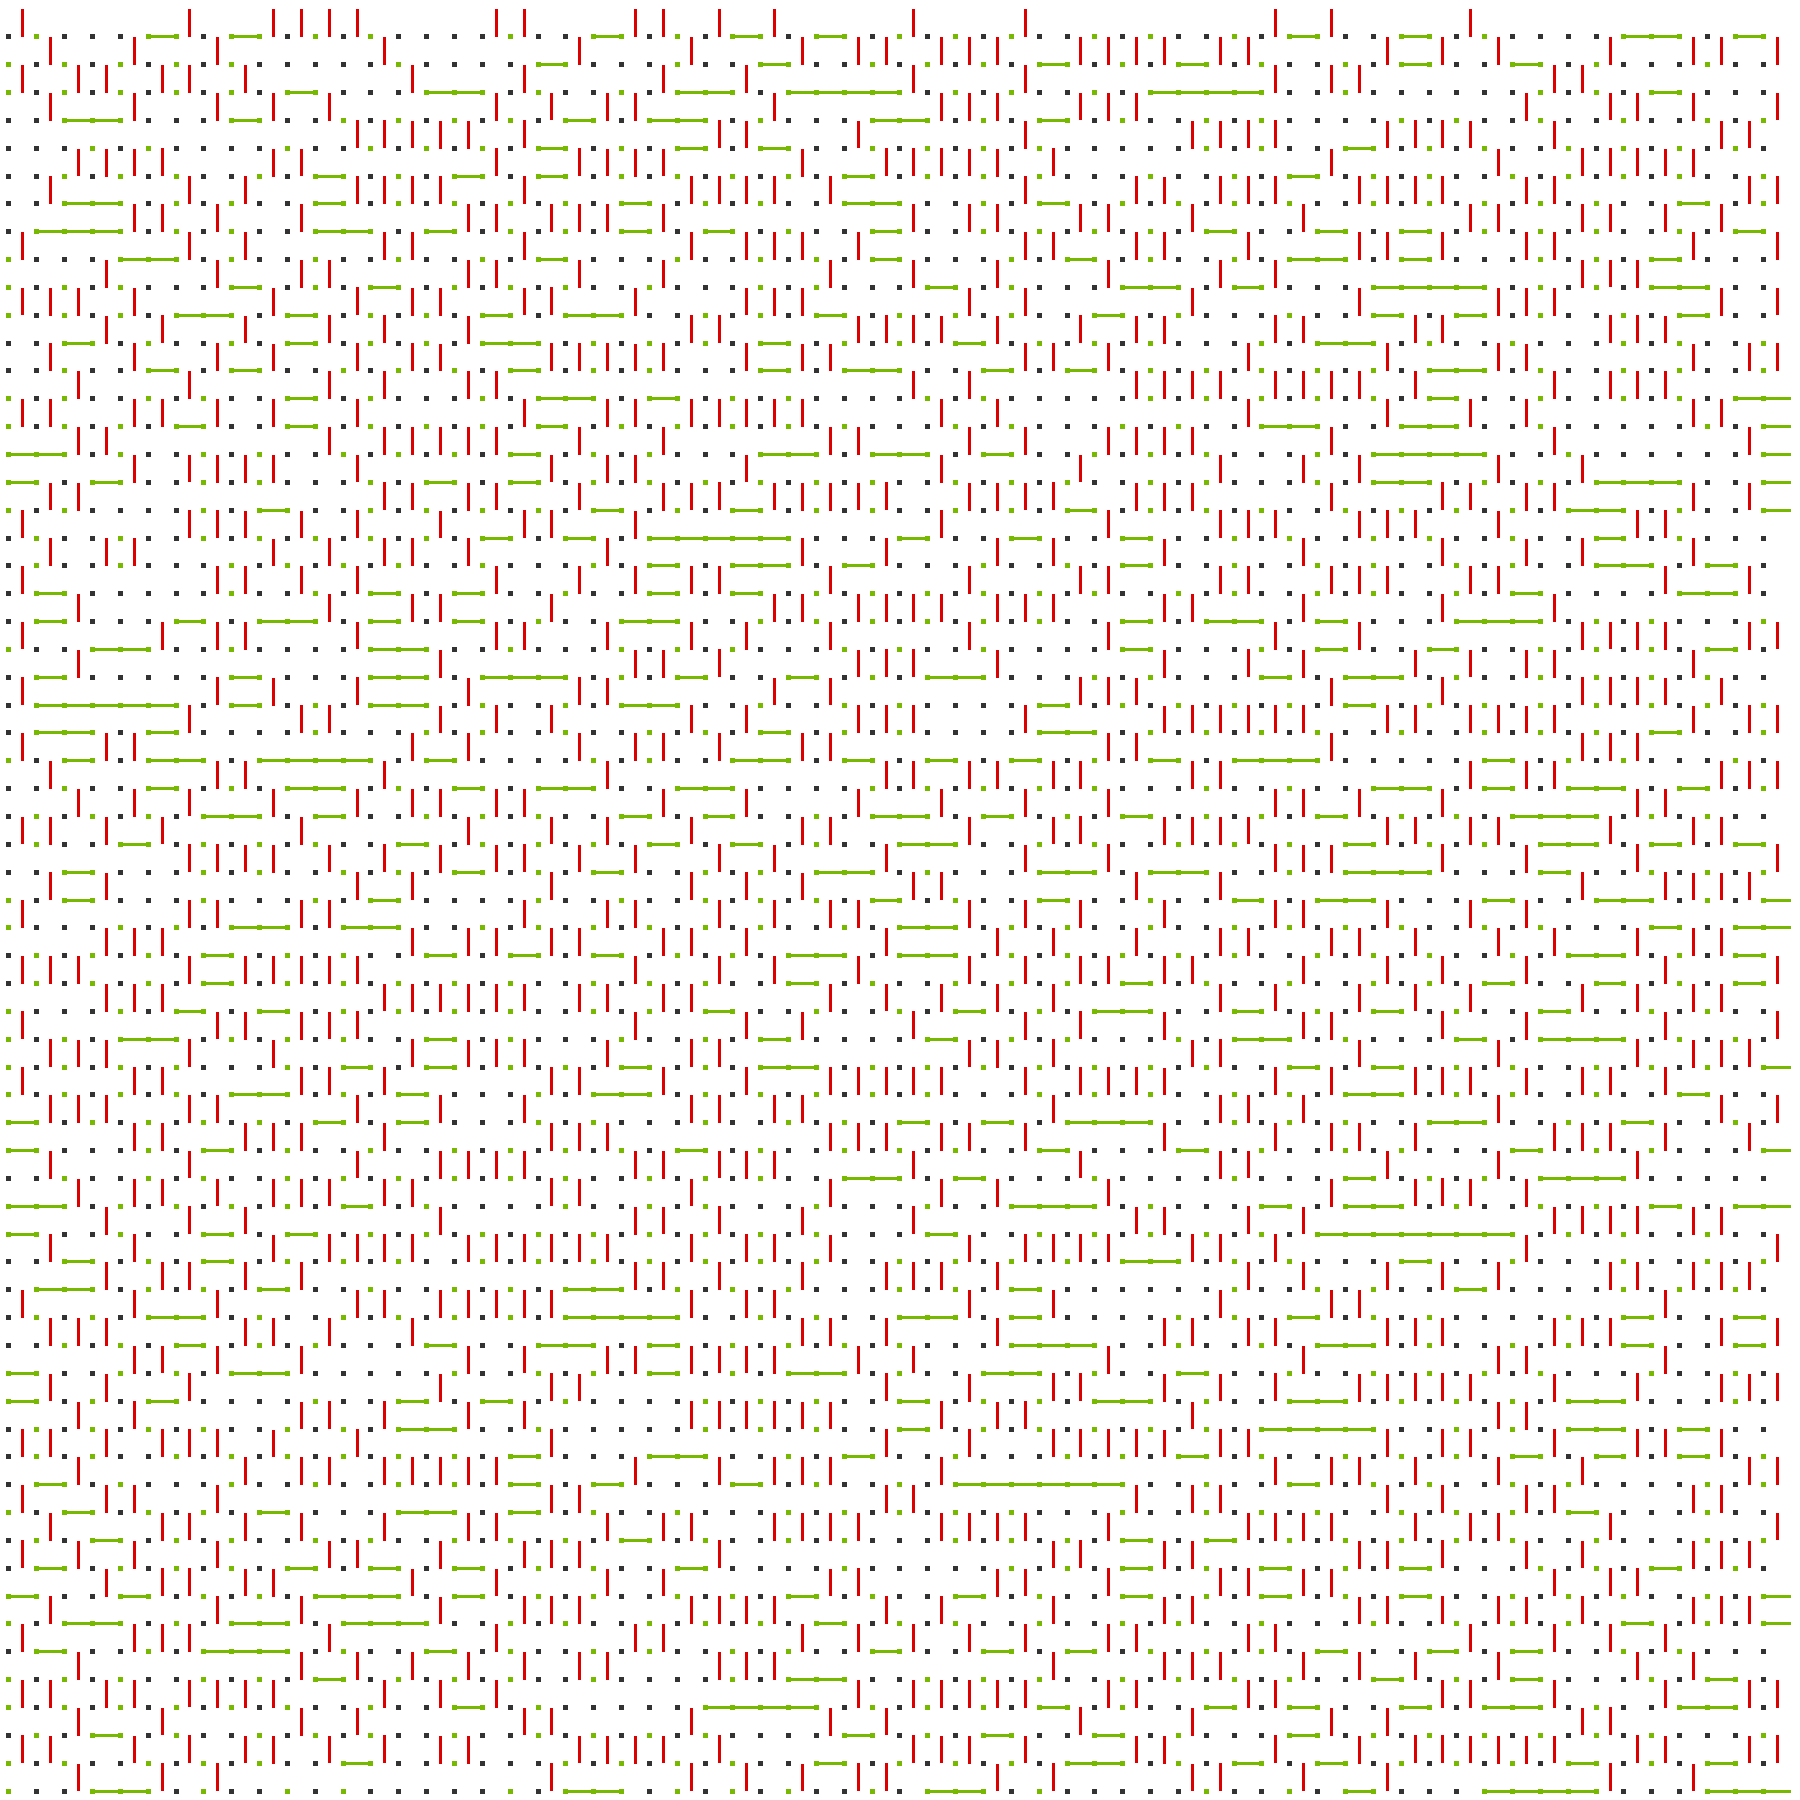
\includegraphics[width=0.3\textwidth]{figs/0.01.png}}\hspace{12mm}
    \subfloat[$h=0.5$.]{
      \label{fig:0.5}
      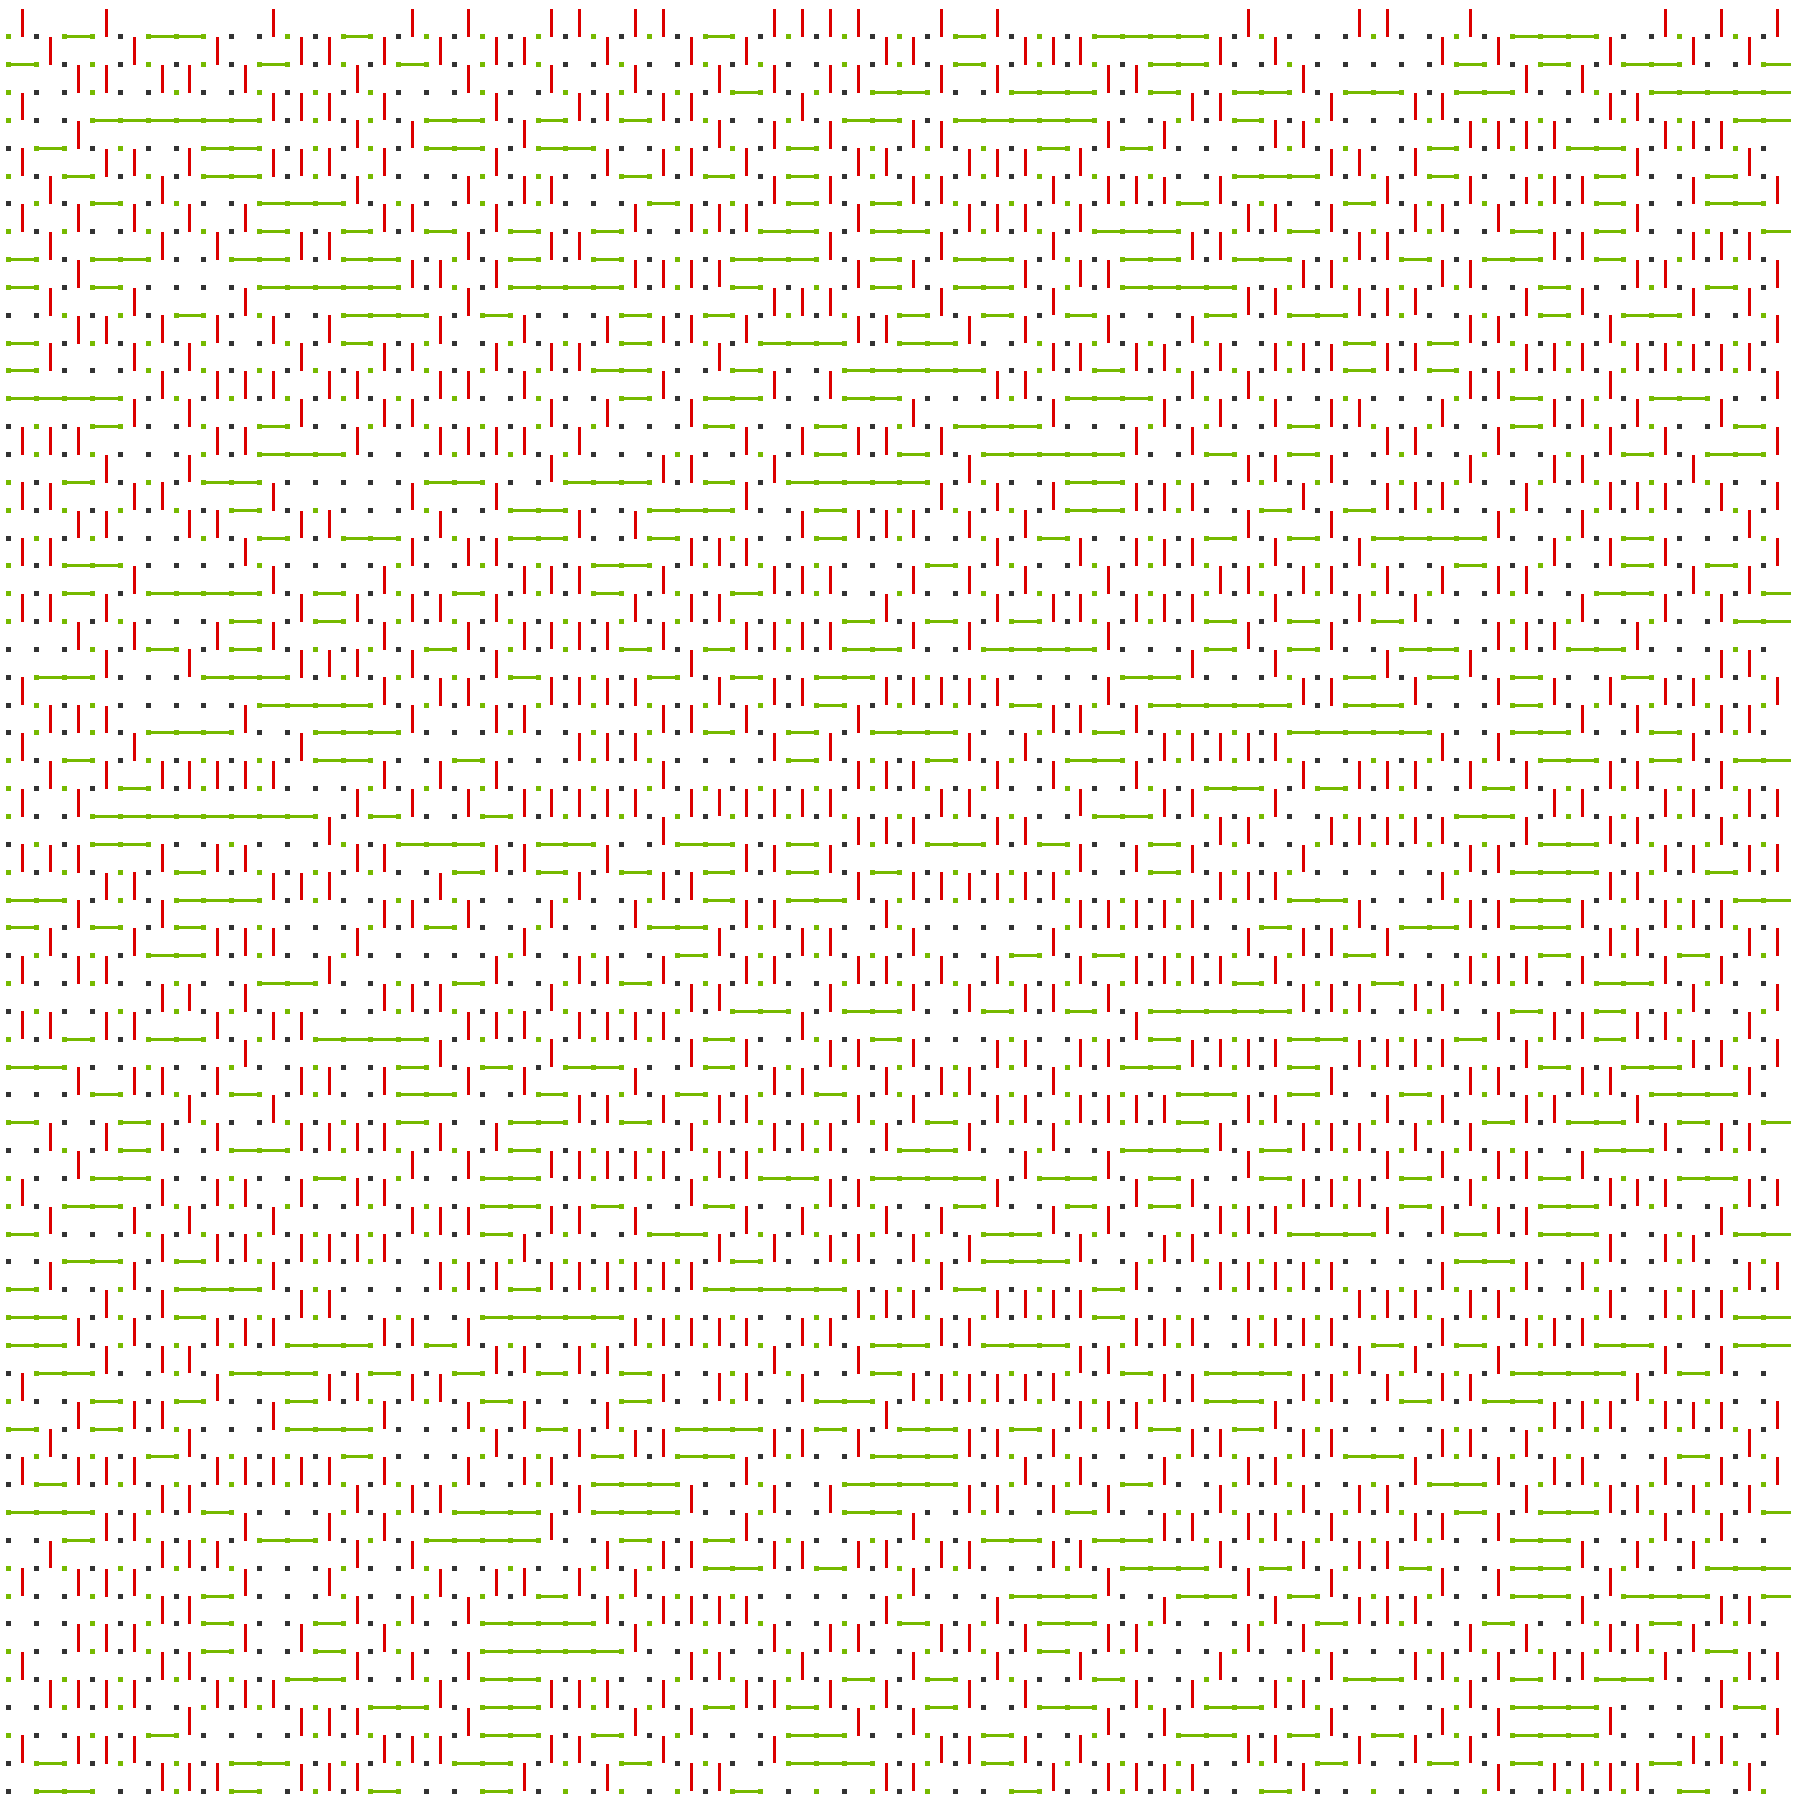
\includegraphics[width=0.3\textwidth]{figs/0.5.png}}\\
    \vspace{-3mm}
    \subfloat[$h=1.0$.]{
      \label{fig:1.0}
      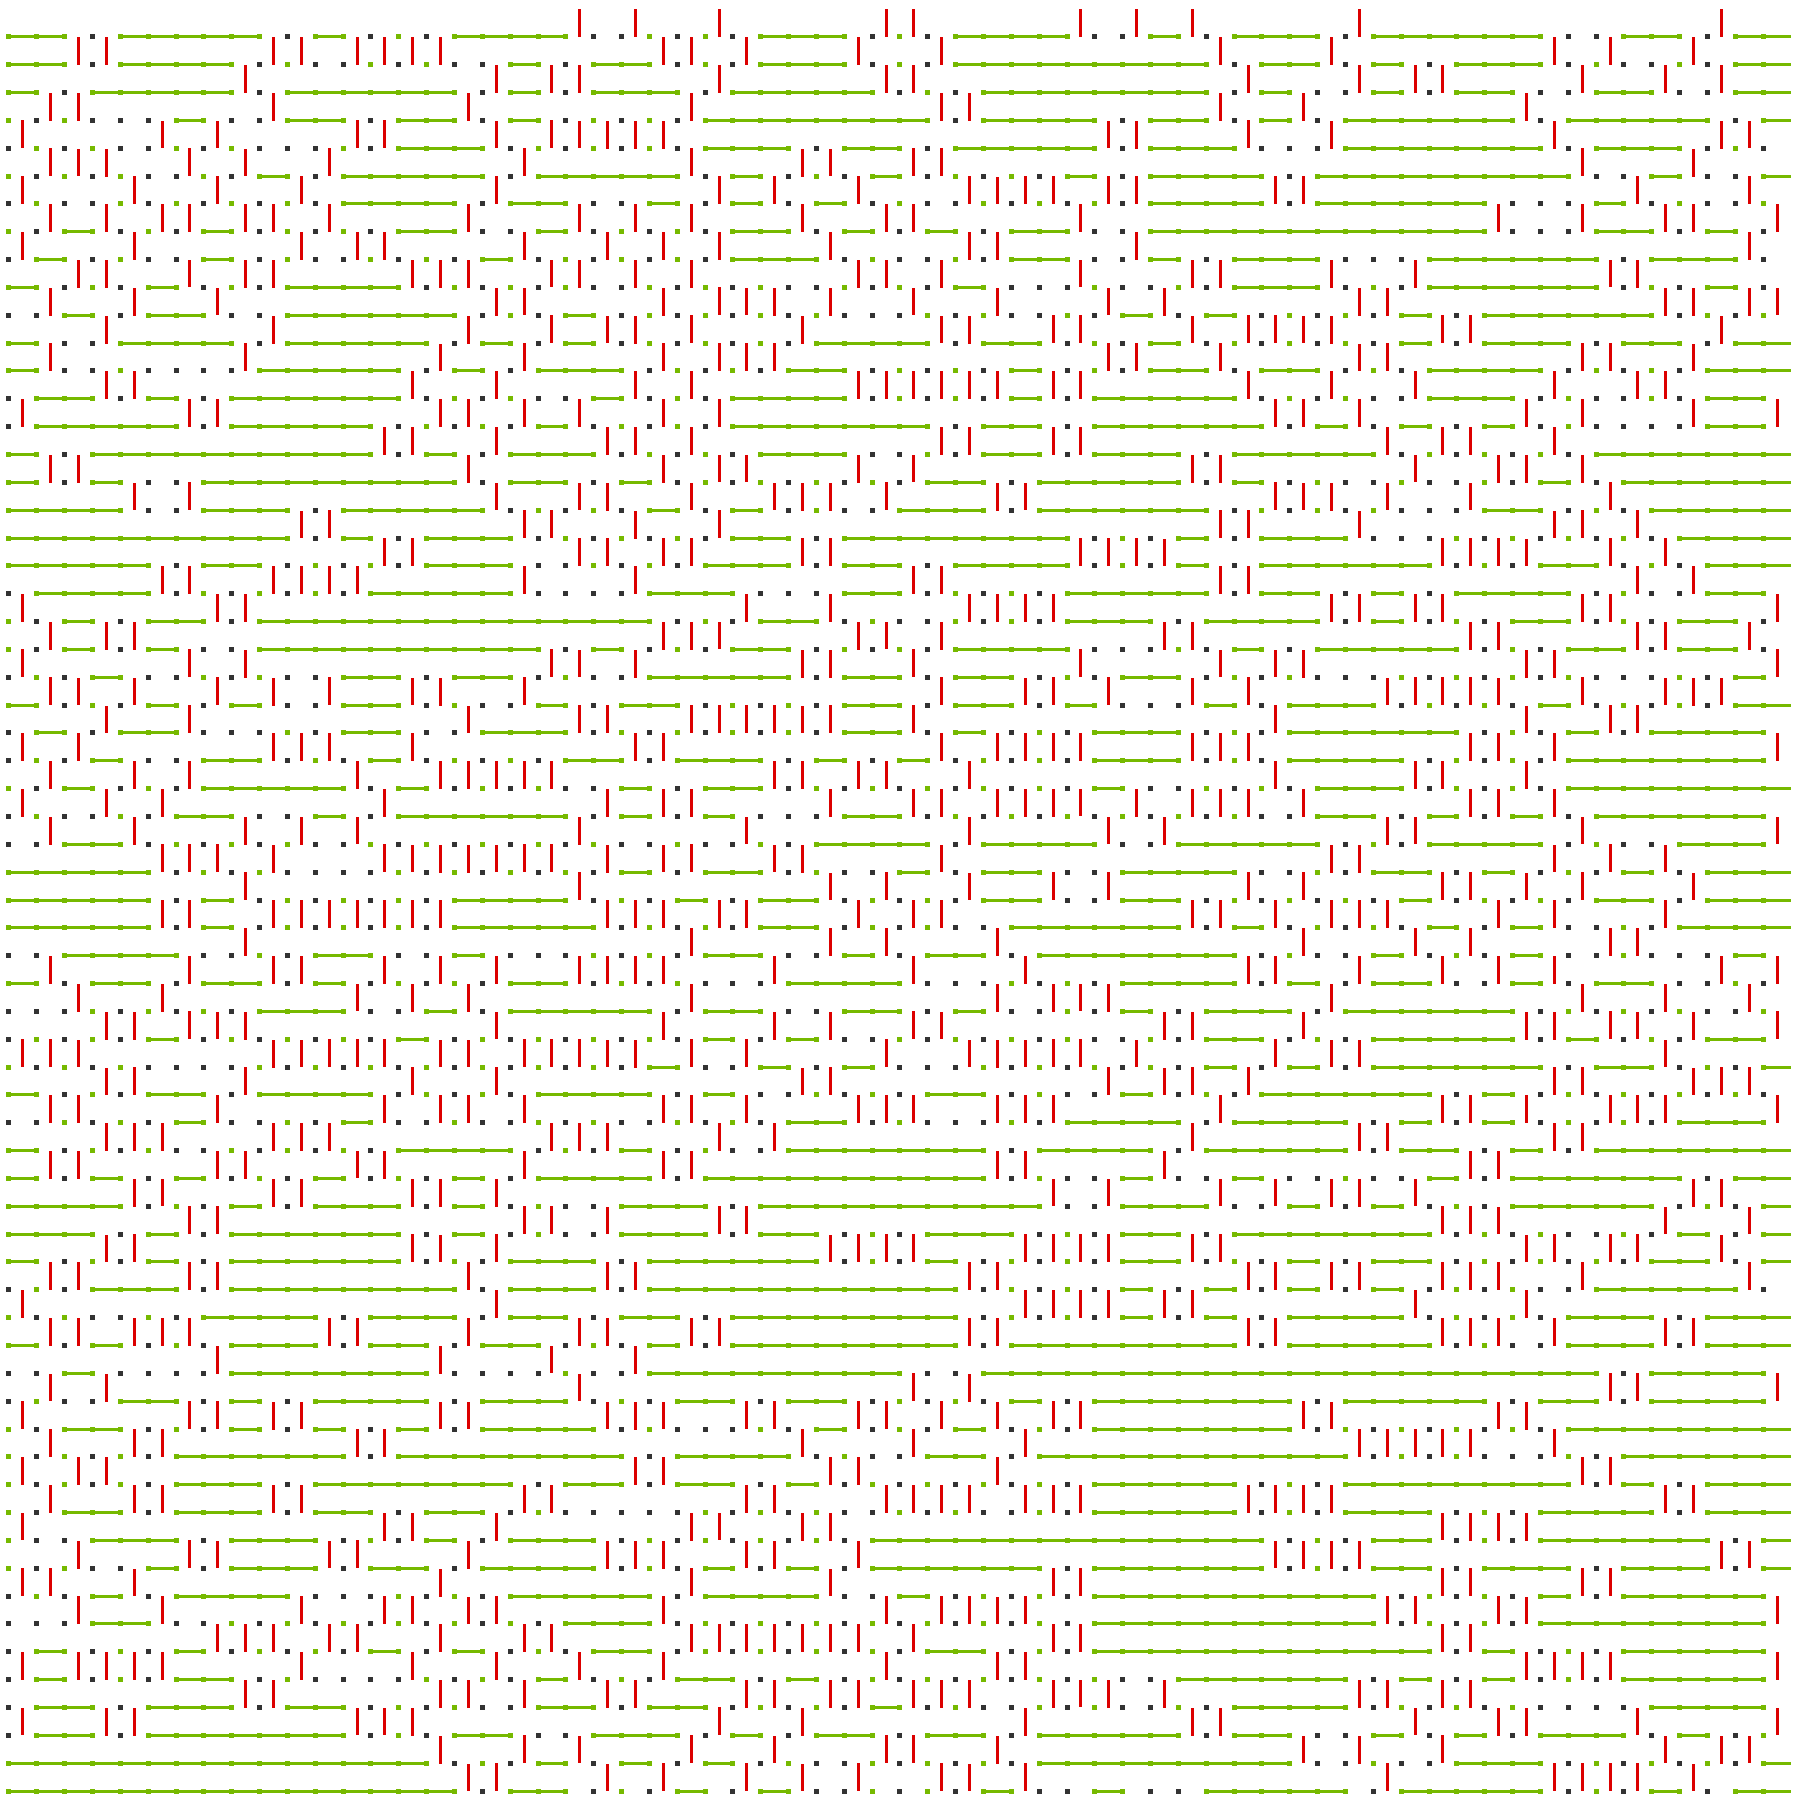
\includegraphics[width=0.3\textwidth]{figs/1.0.png}}\hspace{12mm}
    \subfloat[$h=1.5$.]{
      \label{fig:1.5}
      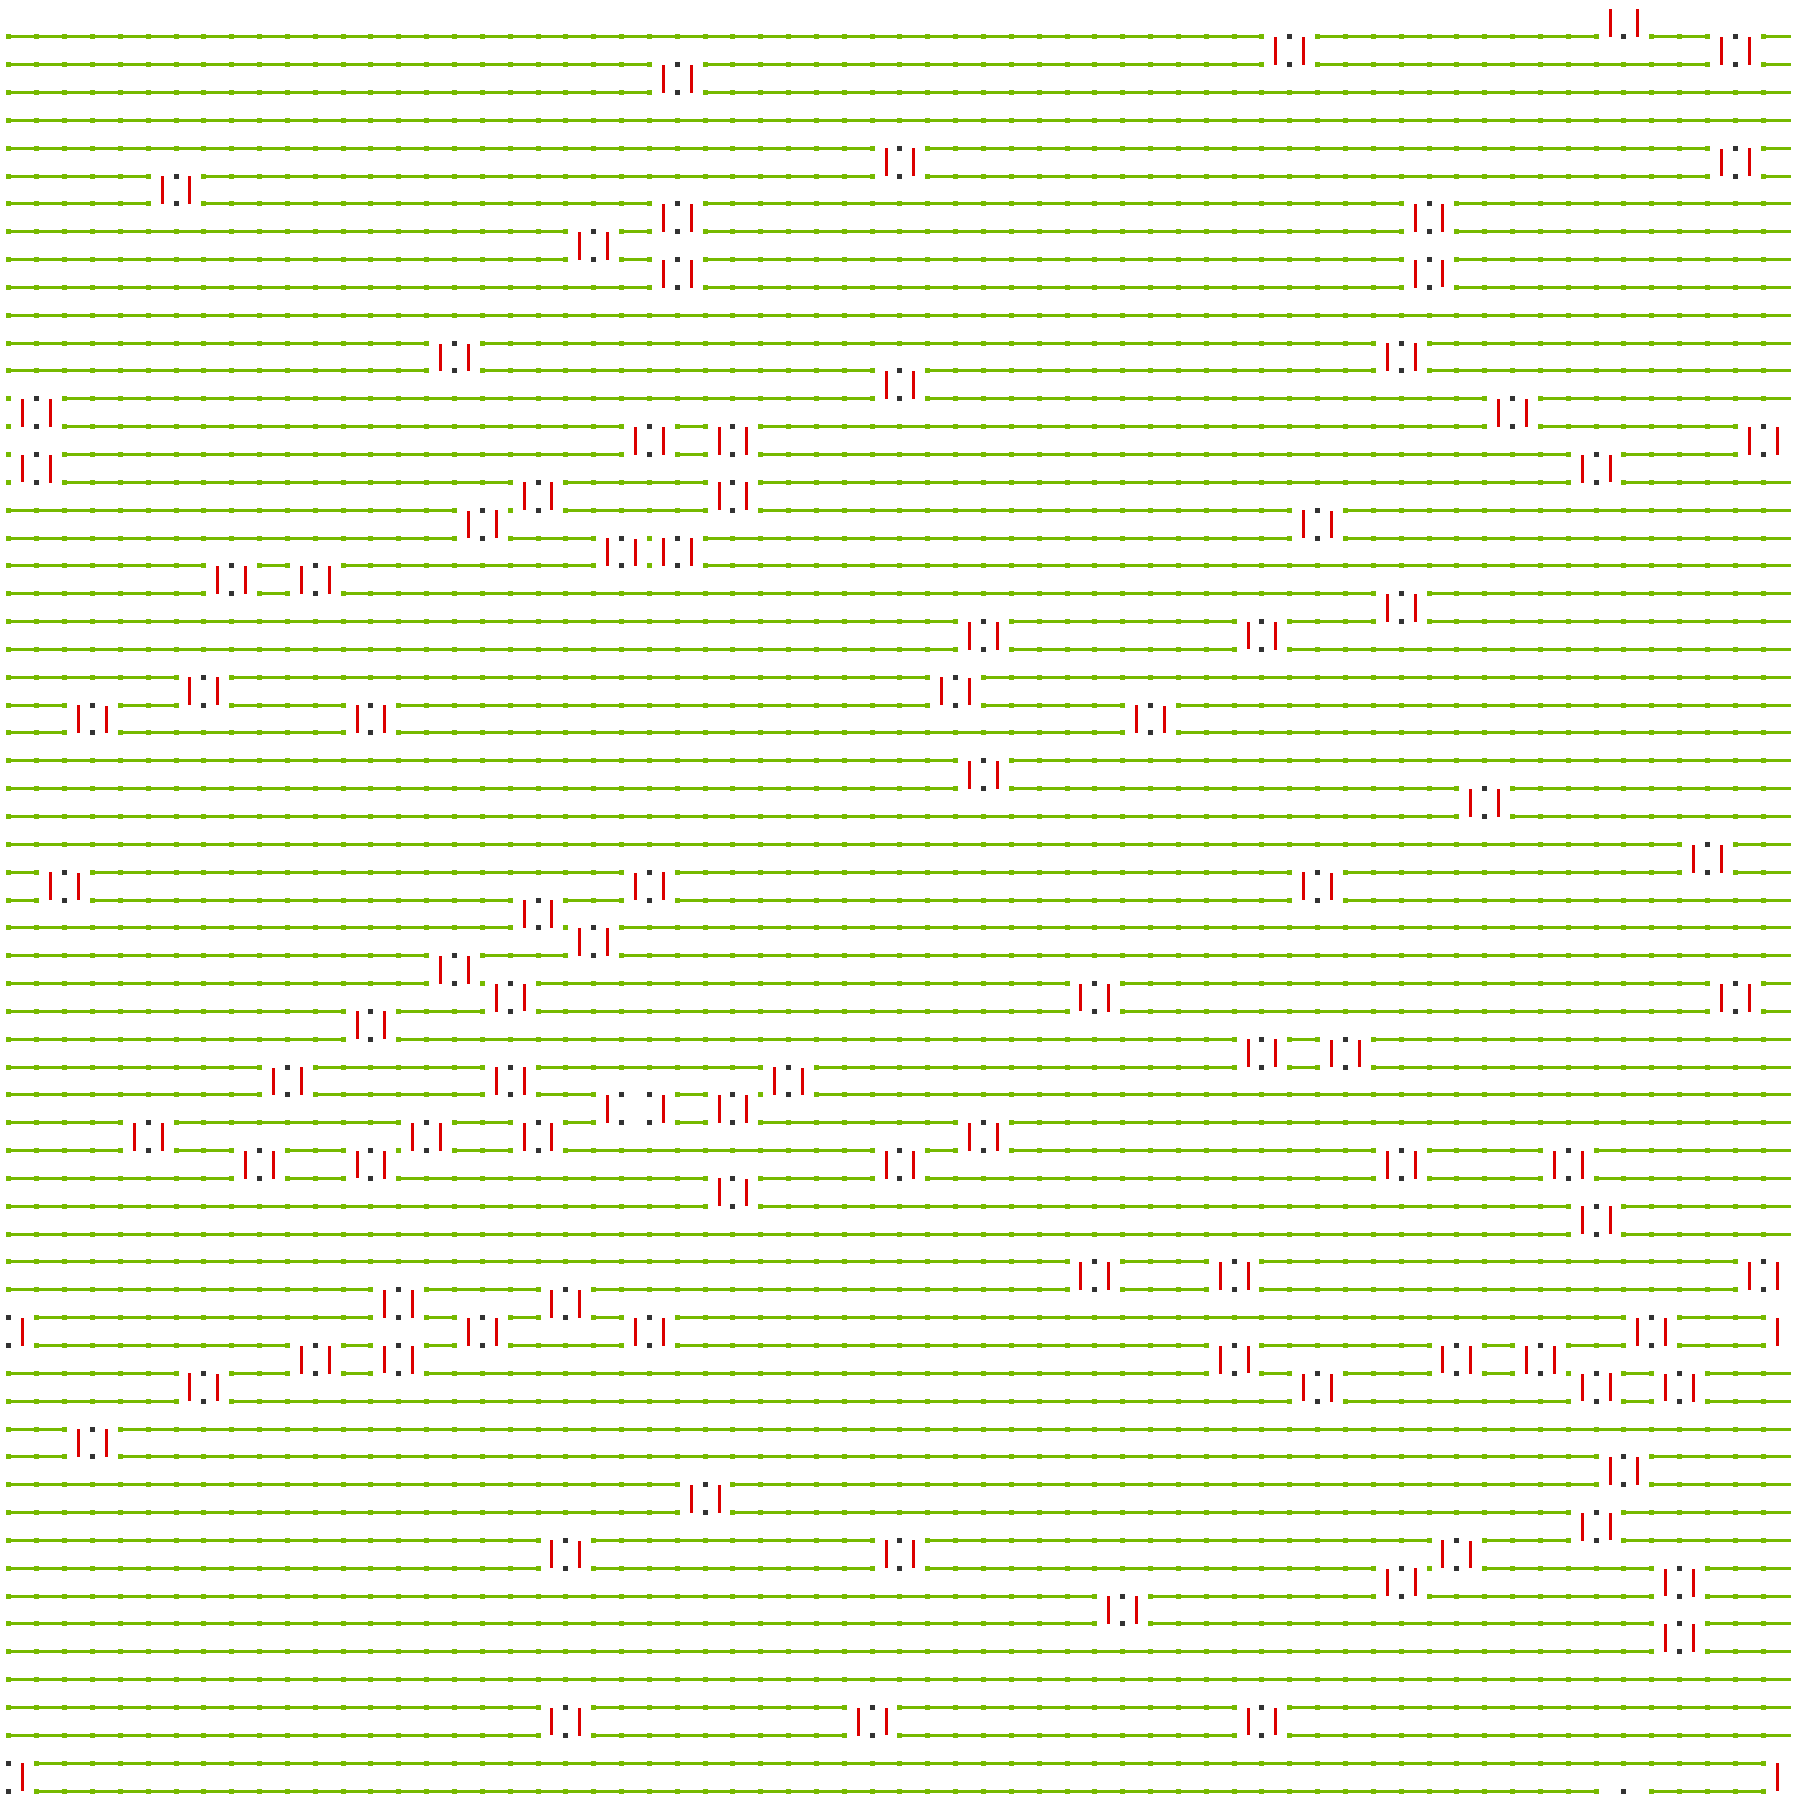
\includegraphics[width=0.3\textwidth]{figs/1.5.png}}
  \end{figure}
\end{frame}

\begin{frame}{Calculated quantities}
  \begin{itemize}
    \item Topological quantities: winding number $W^l$ $\Rightarrow$ total winding number $W$ $\Rightarrow$ wrapping probability $R$.
    \item Physical quantities: correlation functions.
      \begin{gather*}
        \overline{\sigma_i^z} \equiv \frac{1}{L^2}\sum_{j,k}\sigma_{j,k}^z,\\
        \overline{\sigma_i^z \sigma_{i+n}^z} \equiv \frac{1}{L^2} \sum_{j,k}\sigma_{j,k}^z \sigma_{j+n,k}^z,\\
        C_n \equiv \overline{\sigma_i^z \sigma_{i+n}^z}-\overline{\sigma_i^z}^2,
      \end{gather*}
  \end{itemize}
\end{frame}

\begin{frame}{Wrapping Probabilities}
  \begin{figure}[htpb]
    \centering
    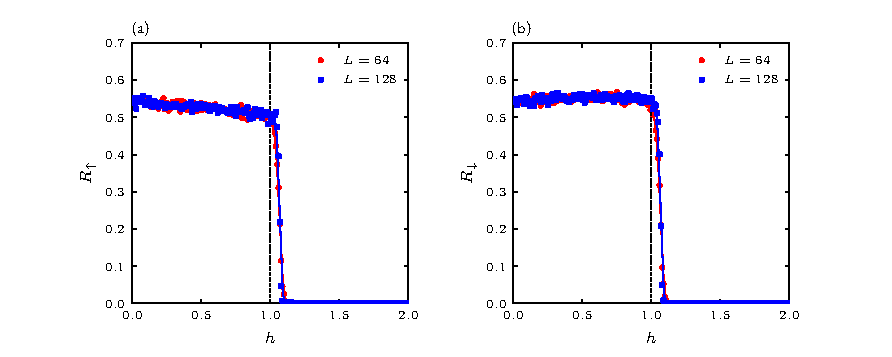
\includegraphics[width=1.3\textwidth,center]{figs/wrapping_probability.pdf}
    \caption{Wrapping probabilities $R_\uparrow$ and $R_\downarrow$ versus the transverse field $h$. (a) Spin-up. (b) Spin-down.}
    \label{fig:wrapping_probability}
  \end{figure}
\end{frame}

\begin{frame}{Correlation Functions}
  \begin{figure}[htpb]
    \centering
    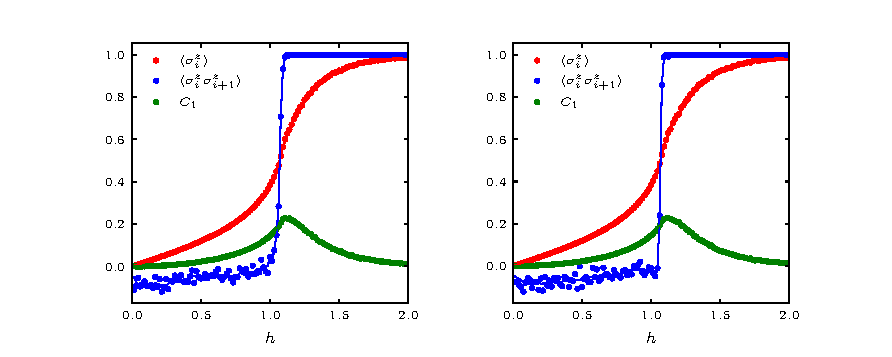
\includegraphics[width=1.3\textwidth,center]{figs/correlation_functions.pdf}
    \caption{Expectation values of spin states $\overline{\sigma_i^z}$, product of NN spins $\overline{\sigma_i^z \sigma_{i+1}^z}$ and correlation function $C_1$ versus transverse field $h$. (a) $L = 64$. (b) $L = 128$.}
    \label{fig:correlation_functions}
  \end{figure}
\end{frame}

\begin{frame}{Correlation Functions}
  \begin{figure}[htpb]
    \centering
    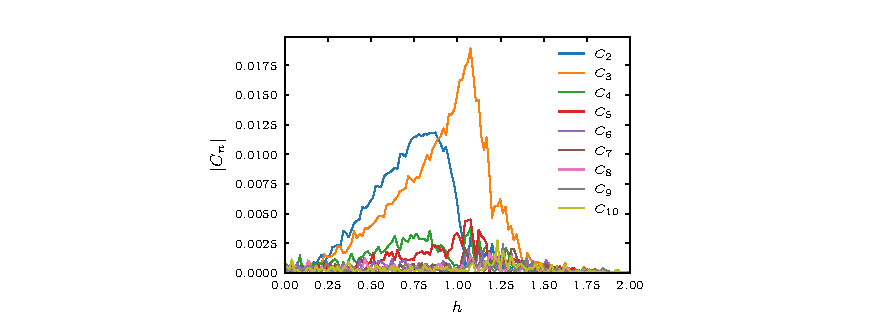
\includegraphics[width=1.5\textwidth,center]{figs/C_n.pdf}
    \caption{Correlation functions $|C_n|$ versus the transverse field $h$.}
    \label{fig:C_n}
  \end{figure}
\end{frame}

\section*{Thanks}
\begin{frame}{}
  \Huge\centering
  \textit{Thank you for listening!}
\end{frame}
\end{document}
